Như đã thảo luận ở phần mạng hồi quy, vấn đề đầu tiên mà chúng ta gặp phải là độ dốc biến mất hoặc độ dốc bùng nổ luôn xảy ra, và ta không thể giải quyết triệt để vấn đề này. Ngoài ra trong mạng hồi quy, như đã nói thì kiến trúc của nó làm cho nó hoạt động giống như một bộ nhớ (vì nó có ghi nhớ thông tin của dữ liệu trước đó), nhưng bộ nhớ này không phải là vô hạn. Và khi chiều dài dữ liệu tăng lên tương đương với việc số lớp tăng lên, thông tin từ dữ liệu cũ ngày càng mất giá trị so với thông tin mới nhận được. Nghĩa là ta có thể nói bộ nhớ này bị quên đi ký ức cũ khi lượng ký ức mới nạp vô càng nhiều. Ví dụ xét một mạng hồi quy khi ta cho học câu dữ liệu sau:\newline
\indent\textit{``Nhà em có nuôi một con chó cỏ. Con chó có đôi mắt to, đôi tai vểnh lên và cái đuôi đen tuyền. Năm nay nó đã 10 tuổi''}\newline
Mạng hồi quy bây giờ sẽ không biết được ``nó'' ở câu thứ ba đang nói về ``con chó cỏ'' ở câu đầu tiên, vì dữ liệu đủ dài sẽ ghi đè và làm xáo trộn dữ liệu, kết quả là làm dữ liệu cũ bị yếu đi đáng kể. Từ đó có thể nói răng mạng thần kinh hồi quy học tốt khi sử dụng dữ liệu chuỗi ngắn, mỗi lần chỉ xử lý duy nhất một dữ liệu, và ta gọi mạng hồi quy có đặc tính của bộ nhớ ngắn hạn (\textit{short-term memory}). Và ngược lại để sử dụng dữ liệu chuỗi dài, hay ta muốn tạo ra một mạng thần kinh có đặc tính của bộ nhớ dài hạn (\textit{long-term memory}), ta phải giải quyết được vấn đề về việc ký ức cũ của bộ nhớ không bị mất đi khi có nhiều ký ức mới. Bộ nhớ dài-ngắn hạn được sinh ra với đặc tính lưu trữ các bộ nhớ ngắn hạn, nhưng trong khoảng thời gian dài hơn.
\begin{figure}[htbp]
    \centering
    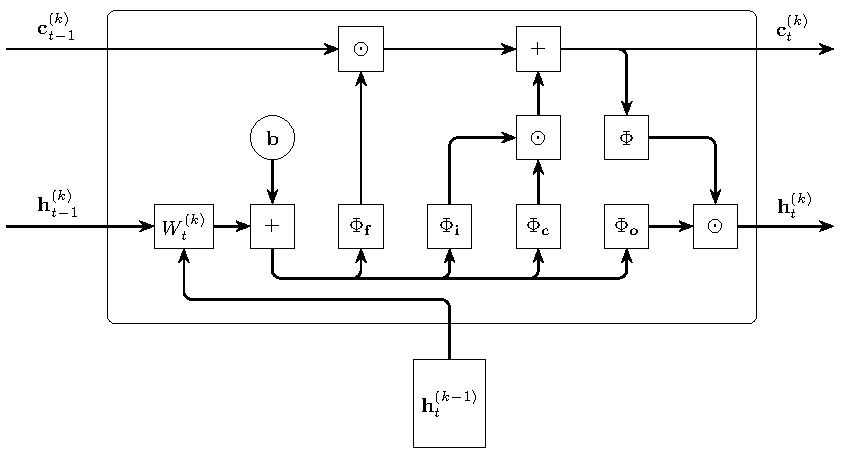
\includegraphics[width=0.7\textwidth]{tikz_image/lstm_architecture.pdf}
    \caption{Kiến trúc của LSTM}
    \label{figure:lstm-architecture}
\end{figure}

Một bộ nhớ dài-ngắn hạn là một phiên bản nâng cấp của mạng hồi quy nhiều lớp với sự tinh chỉnh các bước tính toán ở trong trạng thái ẩn khi nó được lan truyền. Để đạt được điều đó ta thêm vô một trạng thái ẩn khác và gọi trạng thái ẩn mới này là một ô trạng thái (\textit{cell state}) $\mathbf c_t$. Ta có thể xem ô trạng thái này hoạt động như một bộ nhớ thông thường với hai chức năng chính là ``quên'' và ``nhớ''.

Xét một nút ẩn bất kỳ trong mạng thần kinh nhiều lớp, phương trình để tính một trạng thái ẩn bất kỳ được đề cập ở \ref{equation:rnn-multi-layer} chỉ dùng một phép nhân ma trận, với bộ nhớ dài-ngắn hạn thì trạng thái ẩn được tính phức tạp hơn. Gọi $\mathbf{i,f,o,c}$ là bốn vector tức thời khác nhau thể hiện cho đầu vào (\textit{input}), quên (\textit{forget}), đầu ra (\textit{output}), ô trạng thái (\textit{cell state}). Ta có thể xem ba vector $\mathbf{i,f,o}$ là ba cổng logic (\textit{logic gate}). Ba cổng này không mang thông tin mà chỉ hoạt động với mục đích là có cho phép nhận đầu vào hay không (\textit{input gate}), có cho phép quên ký ức cũ hay không (\textit{forget gate}), và có cho phép kết hợp với đầu ra hay không (\textit{output gate}). Với vector $\mathbf c$ là bộ nhớ tức thời của lớp này, ta có phương trình tính toán trong lớp
\begin{align}
    \begin{bmatrix}
        \mathbf i \\
        \mathbf f \\
        \mathbf o \\
        \mathbf c
    \end{bmatrix}
                      & =\begin{pmatrix}
                             \text{sigmoid} \\
                             \text{sigmoid} \\
                             \text{sigmoid} \\
                             \Phi
                         \end{pmatrix}
    \left(W^{(k)}_t
    \begin{bmatrix}
            \mathbf h_{t}^{(k-1)} \\
            \mathbf h_{t-1}^{(k)}
        \end{bmatrix} + \mathbf b
    \right)           & \text{[Tính các vector trung gian]}                                                        \\
    \mathbf c_t^{(k)} & =\mathbf f\odot\mathbf c_{t-1}^{(k)}+\mathbf i\odot\mathbf c & \text{[Tinh chỉnh bộ nhớ]}  \\
    \mathbf h_t^{(k)} & =\mathbf o\odot\Phi(\mathbf c_t^{(k)})                       & \text{[Tính trạng thái ẩn]}
\end{align}

Nếu trạng thái ẩn có số chiều là $p$, thì ma trận $W_t^{(k)}$ bây giờ sẽ có số chiều là $4p\times 2p$, vì nó cần tạo ra bốn vector trung gian ở đầu ra. Bộ nhớ dài ngắn hạt hoạt động qua ba bước như sau (chi tiết trong hình \ref{figure:lstm-architecture}):
\begin{enumerate}
    \item Tính các vector trung gian $\mathbf{i,f,o,c}$.
    \item Tại bước tinh chỉnh bộ nhớ $\mathbf c_t^{(k)}$, có hai sự kiện sẽ xảy ra
          \begin{itemize}
              \item $\mathbf f\odot\mathbf c_{t-1}^{(k)}$ quyết định có quên bộ nhớ cũ $\mathbf c_{t-1}^{(k)}$ hay không.
              \item $\mathbf i\odot\mathbf c$ quyết định có thêm dữ liệu mới $\mathbf c$ vào bộ nhớ hay không.
          \end{itemize}
          tổng của hai sự kiện ``quên'' và ``nhớ'' này tạo nên bộ nhớ mới.
    \item Tính trạng thái ẩn sẽ là sự ``rò rỉ'' từ bộ nhớ $c_t^{(k)}$ qua trạng thái ẩn $h_t^{(k)}$ thông qua cổng đầu ra $\mathbf o$.
\end{enumerate}

Hàm sigmoid khi tính giá trị các vector trung gian có ý nghĩa là tính ra giá trị xác xuất để ta quyết định có nên thực hiện các lệnh như thêm đầu vào (\textit{input}), quên giá trị cũ (\textit{forget}) hay thêm vào đầu ra (\textit{output}). Ta có thể xem các vector trung gian là các cổng logic (\textit{logic gate}) AND thay vì các giá trị thực từ sigmoid để đơn giản hoá sự tính toán. Nhưng trong thực tế ta vẫn phải dùng các hàm tương tự sigmoid vì nó có đạo hàm để tính trong lan truyền ngược.
Xét một bộ nhớ dài-ngắn hạn chỉ có một lớp, ta có
\begin{align}
    c_t=f\cdot c_{t-1}+i\cdot c
\end{align}
Đạo hàm của bộ nhớ ở lớp thời gian $t+1$ so với lớp thời gian $t$ sẽ là $f$, nghĩa là dòng lan truyền ngược đối với bộ nhớ $c_t$ sẽ phụ thuộc hoàn toàn vào $f$. Ta chỉ cần đặt hệ số $\mathbf b_f$ tại bước tính các vector trung gian đủ cao để giá trị của nó sau khi qua hàm sigmoid sẽ gần bằng 1, điều này làm cho vấn đề độ dốc biến mất xảy ra rất chậm.
